\documentclass[tikz,border=8pt]{standalone}
\usepackage[T1]{fontenc}
\usepackage{lmodern}
\usepackage{tikz}
\usetikzlibrary{arrows.meta,positioning}

\begin{document}
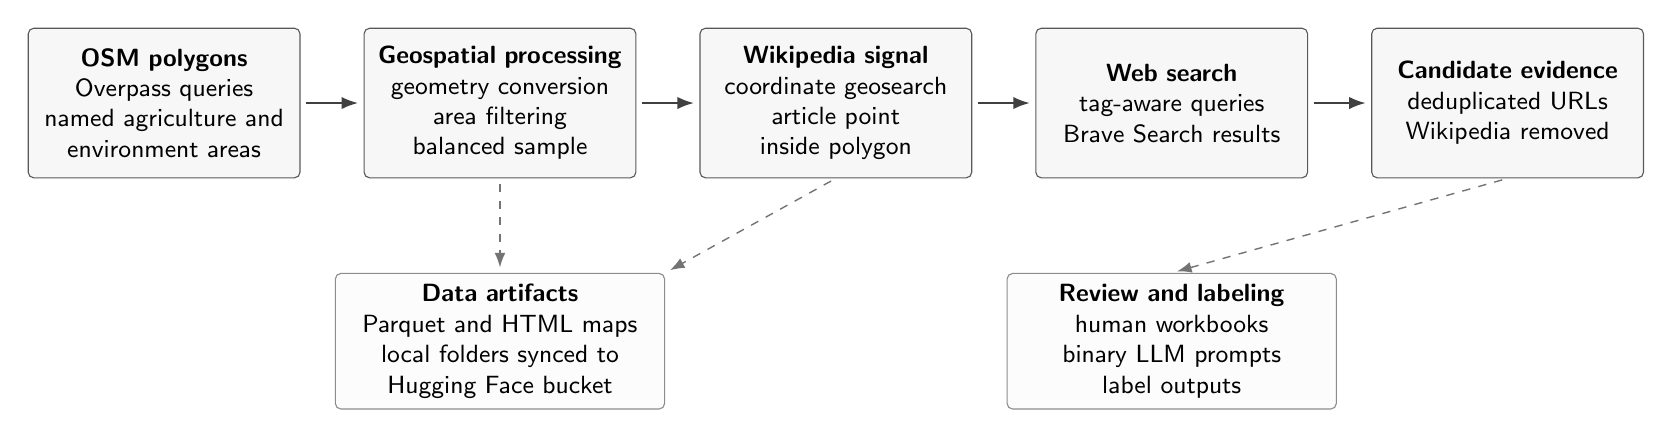
\begin{tikzpicture}[
  font=\sffamily\small,
  >=Latex,
  stage/.style={
    draw=black!65,
    fill=black!3,
    rounded corners=2pt,
    align=center,
    inner sep=5pt,
    minimum height=19mm,
    text width=31mm
  },
  note/.style={
    draw=black!45,
    fill=black!1,
    rounded corners=2pt,
    align=center,
    inner sep=4pt,
    text width=39mm
  },
  arrow/.style={->, line width=.65pt, draw=black!75, shorten >=2pt, shorten <=2pt},
  sidearrow/.style={->, line width=.5pt, draw=black!55, dashed, shorten >=2pt, shorten <=2pt}
]

\node[stage] (osm)
  {\textbf{OSM polygons}\\Overpass queries\\named agriculture and environment areas};

\node[stage, right=8mm of osm] (sample)
  {\textbf{Geospatial processing}\\geometry conversion\\area filtering\\balanced sample};

\node[stage, right=8mm of sample] (wiki)
  {\textbf{Wikipedia signal}\\coordinate geosearch\\article point\\inside polygon};

\node[stage, right=8mm of wiki] (search)
  {\textbf{Web search}\\tag-aware queries\\Brave Search results};

\node[stage, right=8mm of search] (urls)
  {\textbf{Candidate evidence}\\deduplicated URLs\\Wikipedia removed};

\node[note, below=12mm of sample] (storage)
  {\textbf{Data artifacts}\\Parquet and HTML maps\\local folders synced to Hugging Face bucket};

\node[note, below=12mm of search] (eval)
  {\textbf{Review and labeling}\\human workbooks\\binary LLM prompts\\label outputs};

\draw[arrow] (osm) -- (sample);
\draw[arrow] (sample) -- (wiki);
\draw[arrow] (wiki) -- (search);
\draw[arrow] (search) -- (urls);

\draw[sidearrow] (sample.south) -- (storage.north);
\draw[sidearrow] (wiki.south) -- (storage.north east);
\draw[sidearrow] (urls.south) -- (eval.north);

\end{tikzpicture}
\end{document}
